\chapter{Experimentos}

En capítulos anteriores se han expuesto los objetivos marcados para la realización del proyecto así como la solución desarrollada para cada uno de estos problemas y las herramientas utilizadas para las mismas. En este capítulo se muestran los experimentos que se han ido realizando según íbamos cumpliendo objetivos.\\

\section{Simulador Gazebo}

Una vez desarrollado el proyecto y satisfaciendo todos los objetivos marcados se han realizado pruebas sobre la plataforma de simulación Gazebo para comprobar sin ningún tipo de riesgos el funcionamiento del mismo.\\

Para realizar este experimento asemejandose de la manera más realista al experimento final con el drone real se ha utilizado un \emph{Intel Compute Stick}\footnote{\url{http://www.intel.com/content/www/us/en/compute-stick/compute-stick-product-brief.html}} como par local, encargado de conectarse a las interfaces ICE que nos proporciona el plugin ArDrone desarrollado por JdeRobot para el simulador Gazebo. Este ordenador está compuesto por un procesador Intel Atom que corre Ubuntu 14.04 LTS como sistema operativo. El simulador Gazebo se ha ejecutado en el mismo equipo que correrá el navegador remoto, desde el que teledirigimos el drone.\\

Los resultados de este experimento han sido muy positivos, el control y manejo del drone ha sido de manera fluida y sin realizar ningún tipo de movimiento extraño producido por algún tipo de mal-funcionamiento del código. El manejo se ha realizado tanto con los \emph{joysticks} virtuales como con el mando.\\

Una vez superado este experimento se ha realizado el siguiente, consistiendo en realizar pruebas con el drone real.\\

\section{Vuelo del drone real}

Las pruebas con el drone real se han divido a su vez en dos. La primera consiste en realizar las pruebas sin colocar a bordo del drone ni el \emph{computer stick} ni la cámara. Ambos se han usado para las pruebas pero para una primera aproximación se han realizado sin estar a bordo.\\

Así pues la distribución de los equipos es: computer stick como par local, que se conecta al drone real y accede a la cámara USB conectada al mismo, y ordenador portátil como par remoto desde el que se teleoperará el drone y a su vez está ejecutando el servidor de señalización y el \texttt{ardrone\_server.} La figura \ref{fig:experimentodronereal1} muestra la realización de este experimento. En la mediawiki\footnote{\url{http://jderobot.org/Irodmar-tfg#First_Flying_with_Real_Drone}}\cite{Mediawiki} hay un vídeo completo del mismo.\\

\begin{figure}[h!]
\centering
\includegraphics[width=0.9\textwidth]{experimentodronereal1}
\caption{Experimento uno con drone real.}
\label{fig:experimentodronereal1}
\end{figure}

Esta prueba también ha sido un éxito, por lo que nos marcamos el siguiente experimento con el drone y la cámara a bordo del drone. Este experimento la configuración es la misma que en el anterior, pero el manejo del drone con la aplicación será más realista ya que tenemos la cámara en primera persona.\\

*** FIN EXPERIMENTO CON FOTO Y LINK AL VIDEO***


\section{Vuelos con multidispositivos}

Como tercer y último experimento hemos probado a volar el drone utilizando dispositivos móviles. WebRTC tiene soporte para dispositivos móviles y los elementos de control los hemos desarrollado también para dispositivos táctiles, podemos utilizarlos como par remoto, par local o ambos. Al igual que el experimento anterior se ha realizado en dos pasos, primero sin colocar el dispositivo a bordo del drone para confirmar su correcto funcionamiento y posteriormente repitiéndolo con el dispositivo a bordo. Realizar experimentos con dispositivos móviles implica la necesidad de la utilización de un ordenador de apoyo que será el que ejecute tanto el servidor de señalización para WebRTC cómo \emph{ardrone\_server}.\\

Como primer experimento se ha utilizado un ordenador como par local y un móvil como par remoto desde el que gobernamos los movimientos del drone. En la figura \ref{fig:experimentodronemultidispositivo1} se puede apreciar un momento del vídeo del experimento\footnote{url{http://jderobot.org/Irodmar-tfg\#Flying_with_a_mobile_like_Remote_PC}}.\\

\begin{figure}[h!]
\centering
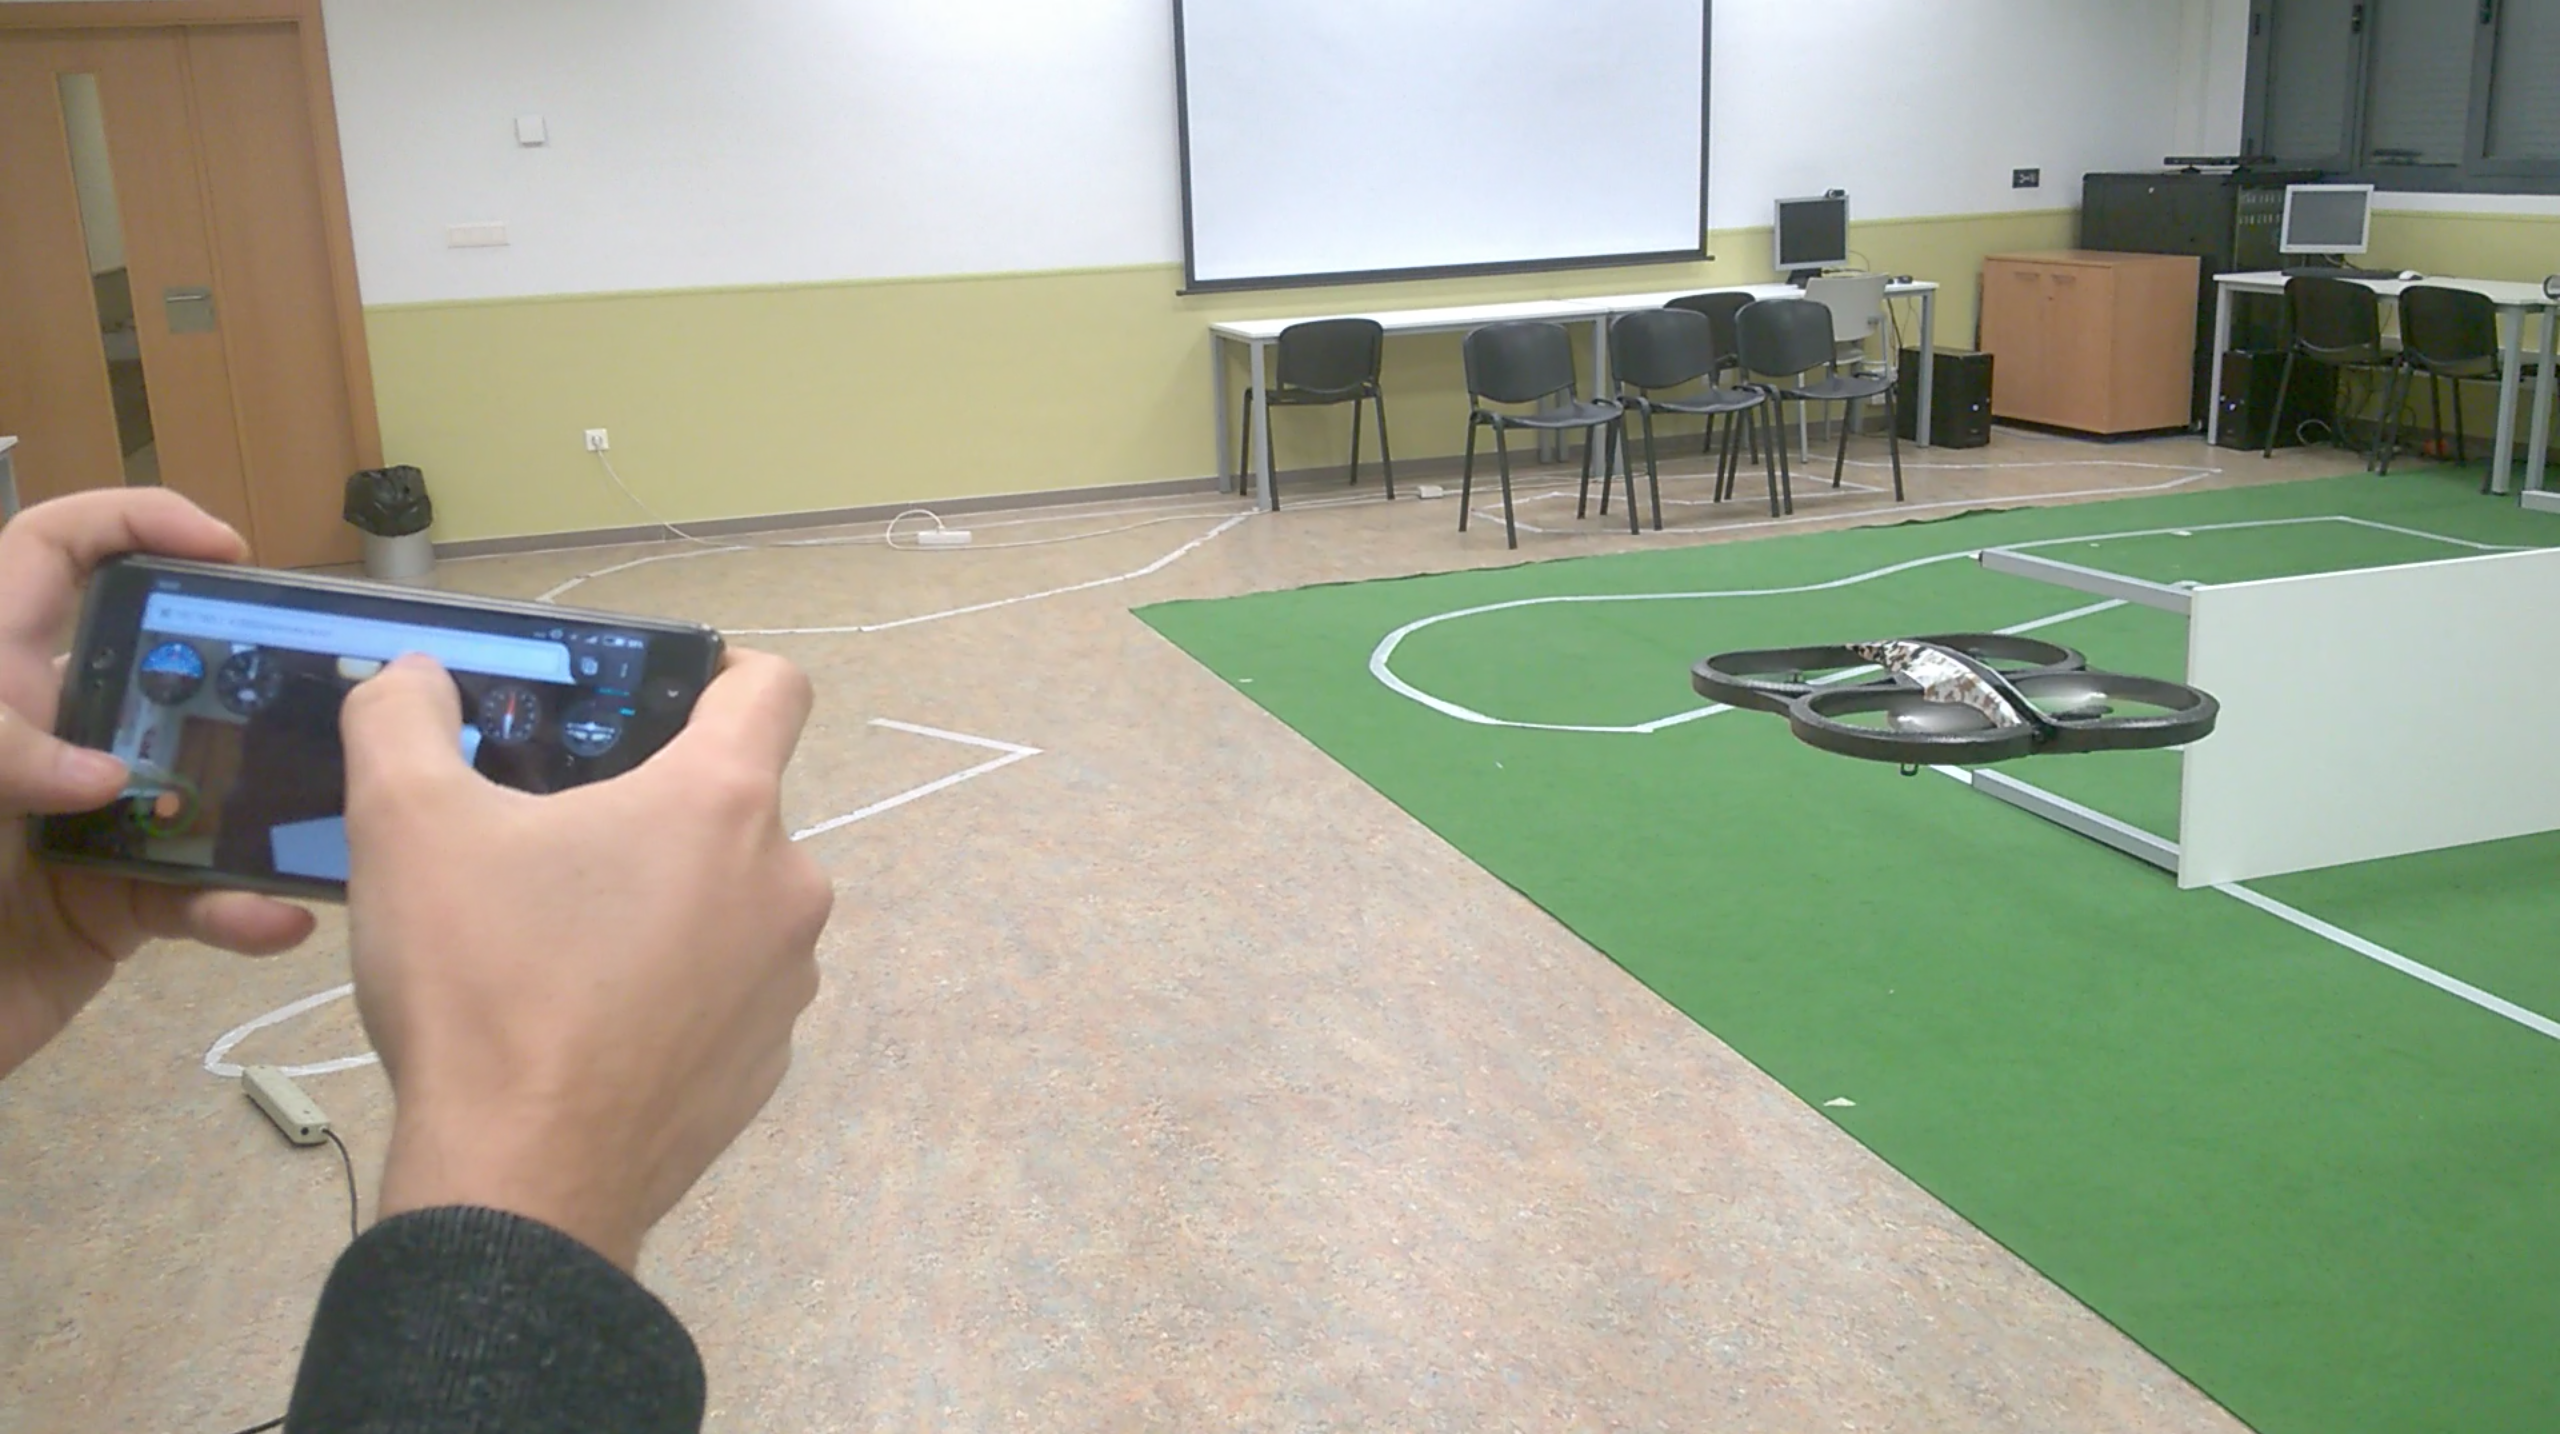
\includegraphics[width=0.9\textwidth]{experimentodronemultidispositivo1}
\caption{Experimento con móvil como par remoto.}
\label{fig:experimentodronemultidispositivo1}
\end{figure}

El segundo experimento es a la inversa, se utiliza un ordenador como par remoto y un dispositivo móvil como par local, encargándose de establecer la conexion con el drone. En este caso las imágenes que se envían son las de cualquieras de las dos cámaras del móvil, la delantera o la trasera. La figura \ref{fig:experimentodronemultidispositivo2} muestra un momento del experimento que esta recogido en un vídeo en la mediawiki\footnote{http://jderobot.org/Irodmar-tfg\#Flying_with_a_mobile_like_Droner_PC}.\\

\begin{figure}[h!]
\centering
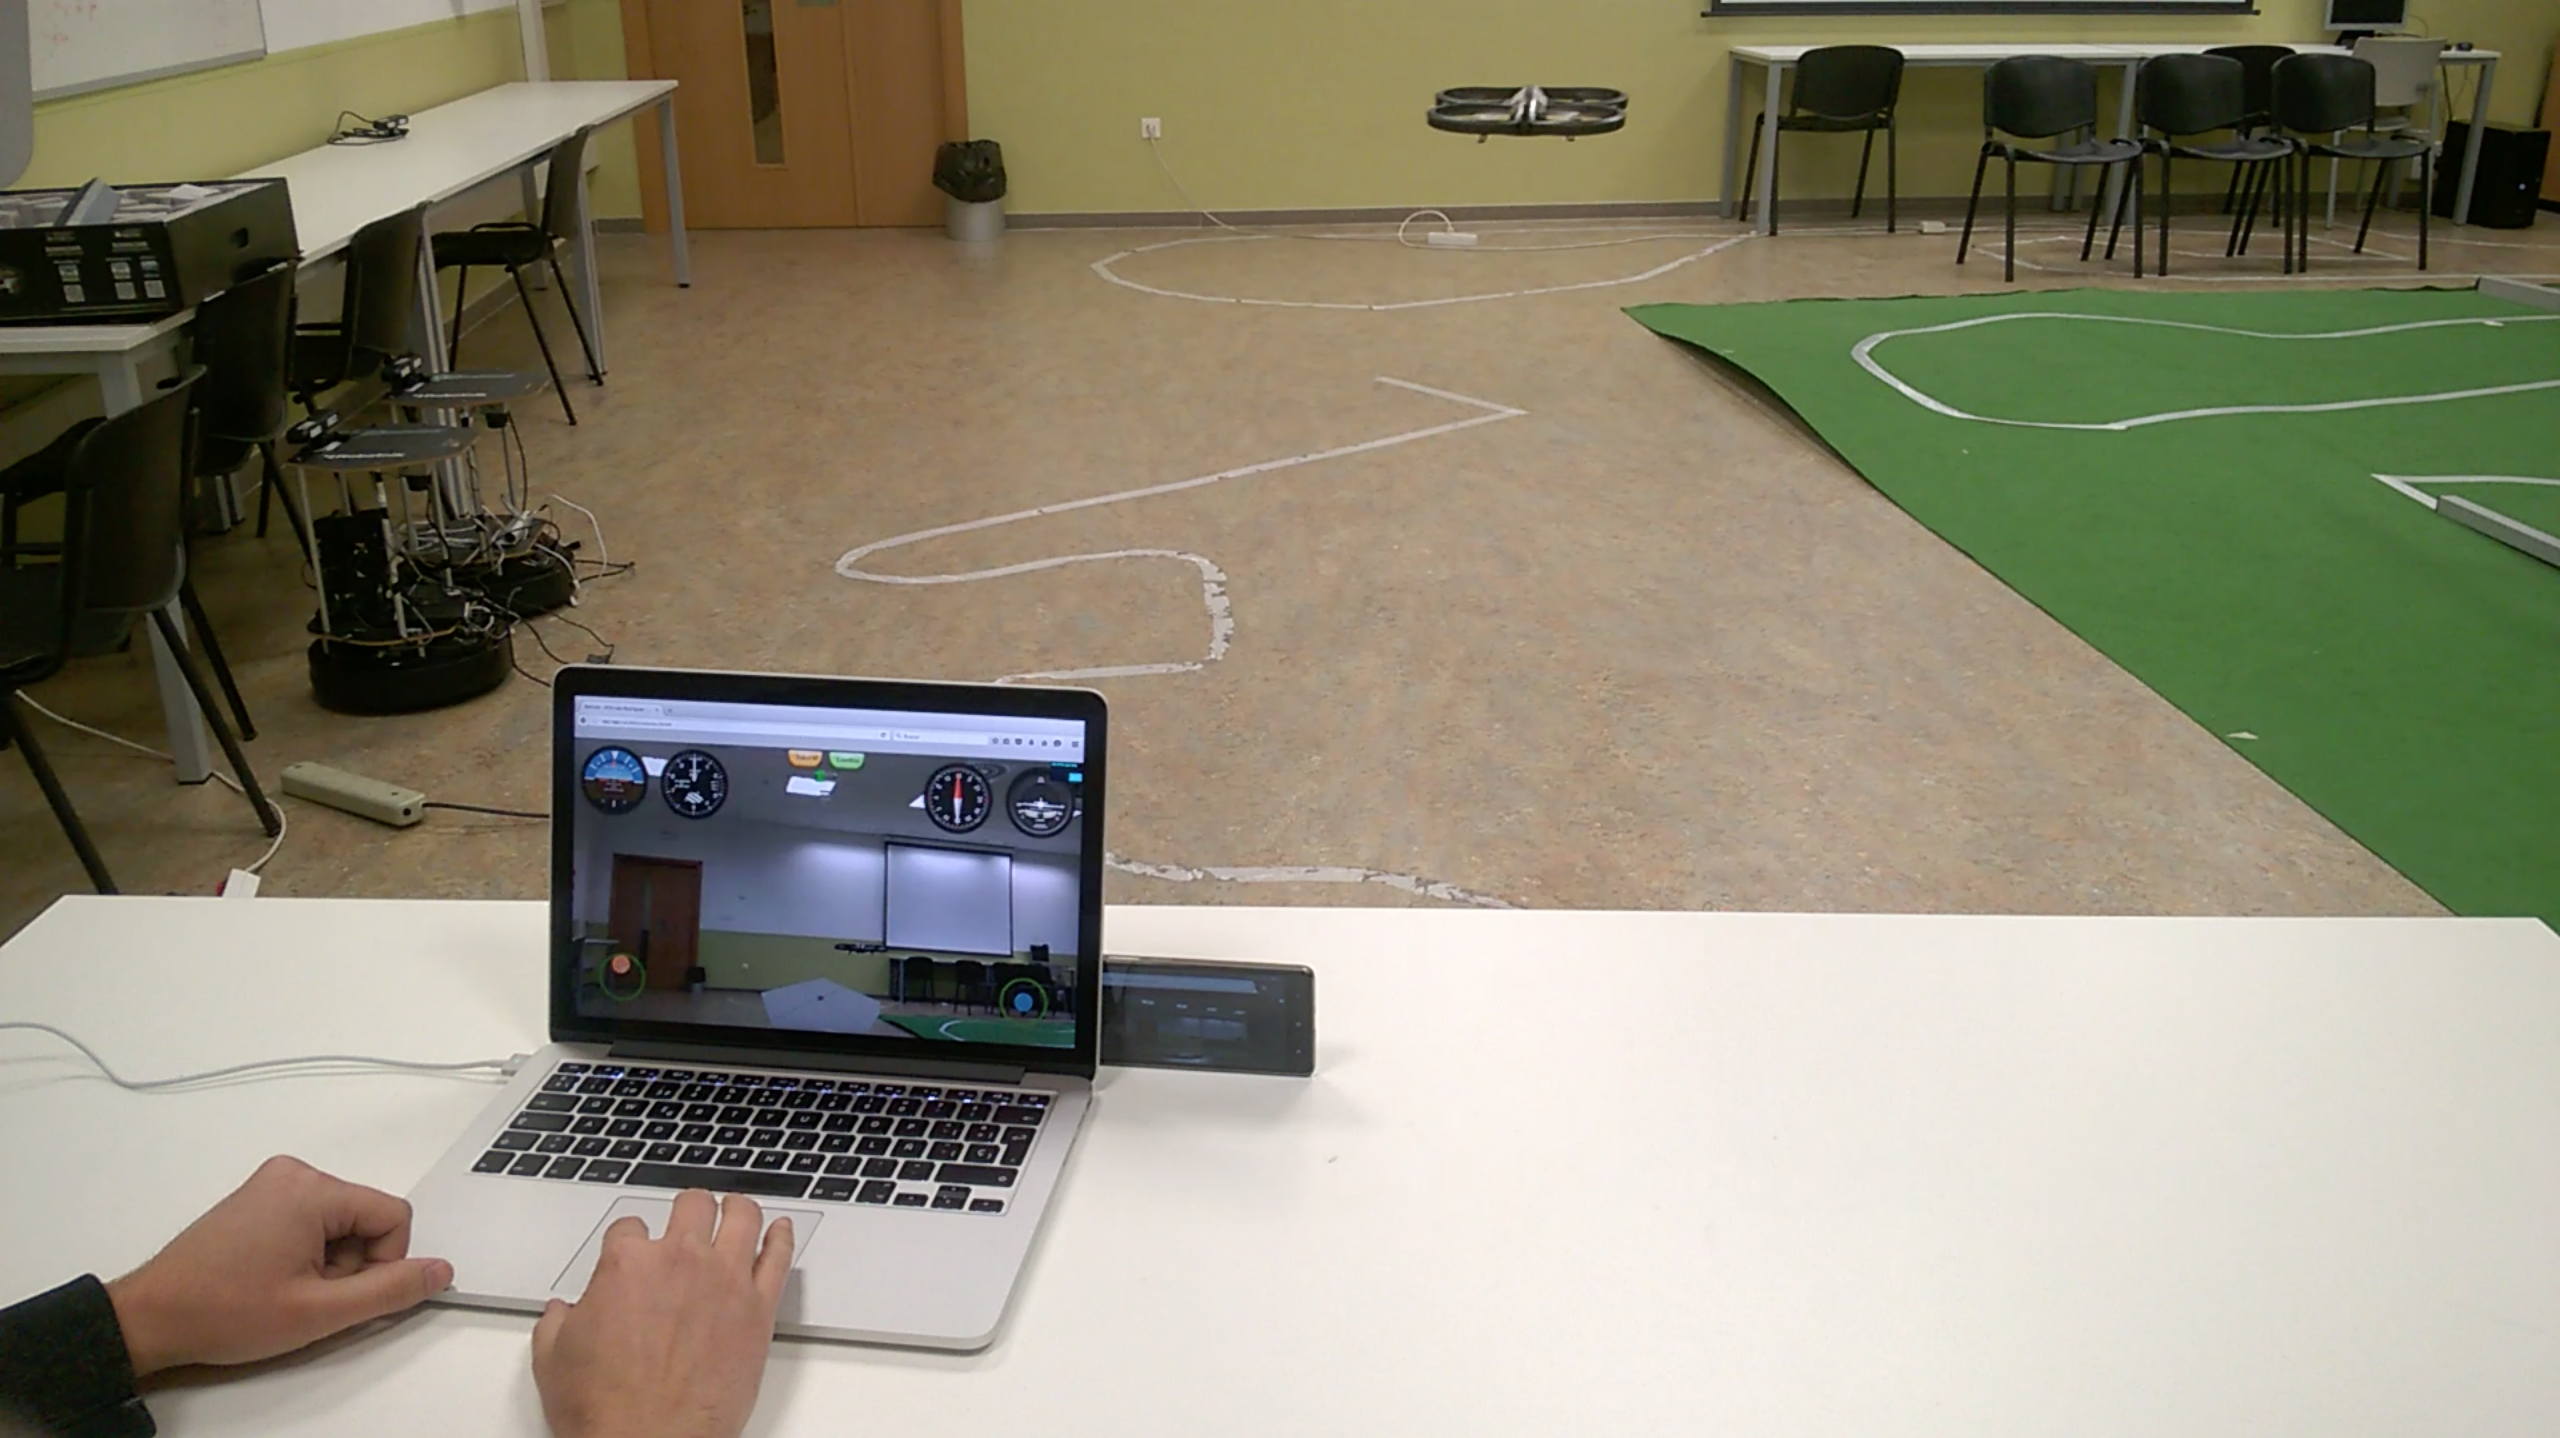
\includegraphics[width=0.9\textwidth]{experimentodronemultidispositivo2}
\caption{Experimento con móvil como par local.}
\label{fig:experimentodronemultidispositivo2}
\end{figure}